% !TeX root = ../Tex/main.tex

\subsection{Robustness}
\subsubsection{Bandwidth}
Process of selection of optimal window of observation has been extensively studied. Nowadays, most statistical softwares provide command that run optimisation process to automatically select the window.

\vspace*{1em}
\textcite{imbensIdentificationEstimationLocal1994} discourges the use of high-order polynomials in the to estame the LATE, they argue that "higher-order polynomials can lead to overfitting and have been found to introduce bias". In the previous pages (\label{sec:overfitting}) we already highlighted the role of overfitting. In particular, we highlighted the contributionof \textcite{cranmerWhatCanWe2017}.

A way of overcoming the issue of overfitting is using nonparametric kernels \parencite[chap.\(\backsim\) 6.2.3]{cunninghamCausalInferenceMixtape2021}. However, in this method the selection of bandwidth is crucial. In fact, it "is sensitive to the choice of bandwidth, but more recent work allows the researcher to estimate optimal bandwidths \textcite{imbensOptimalBandwidthChoice2012,calonicoRobustNonparametricConfidence2014}."

Another issue, namely estimation function, is not stritly related to bandwidth selection. However, \textcite{leeRegressionDiscontinuityDesigns2010} stress the importance of this step. They argue that "allowing different functions on both sides of the discontinuity should be the main results in an RDD paper".

\subsubsection{Manipulation Tests}
In order to strengthen the support to results, I conducted a McCrary Density Test. This test was introduced by \textcite{mccraryManipulationRunningVariable2008}. This test reduces the probability that treated unites "manipulat" the cutoff. In this case it makes us sure of the fact that there is no anticipation effect from Parliament Members. Parliament Members of a party could have decided to rintroduce the reform only when they became sure of having acquired the majority of new voters. This would violate the assumptions that lay at the basics of the regression discontinuity design.
The test, conducted for both cabinet and non cabinet, shows that \textit{there is no manipulation}.

\begin{center}
    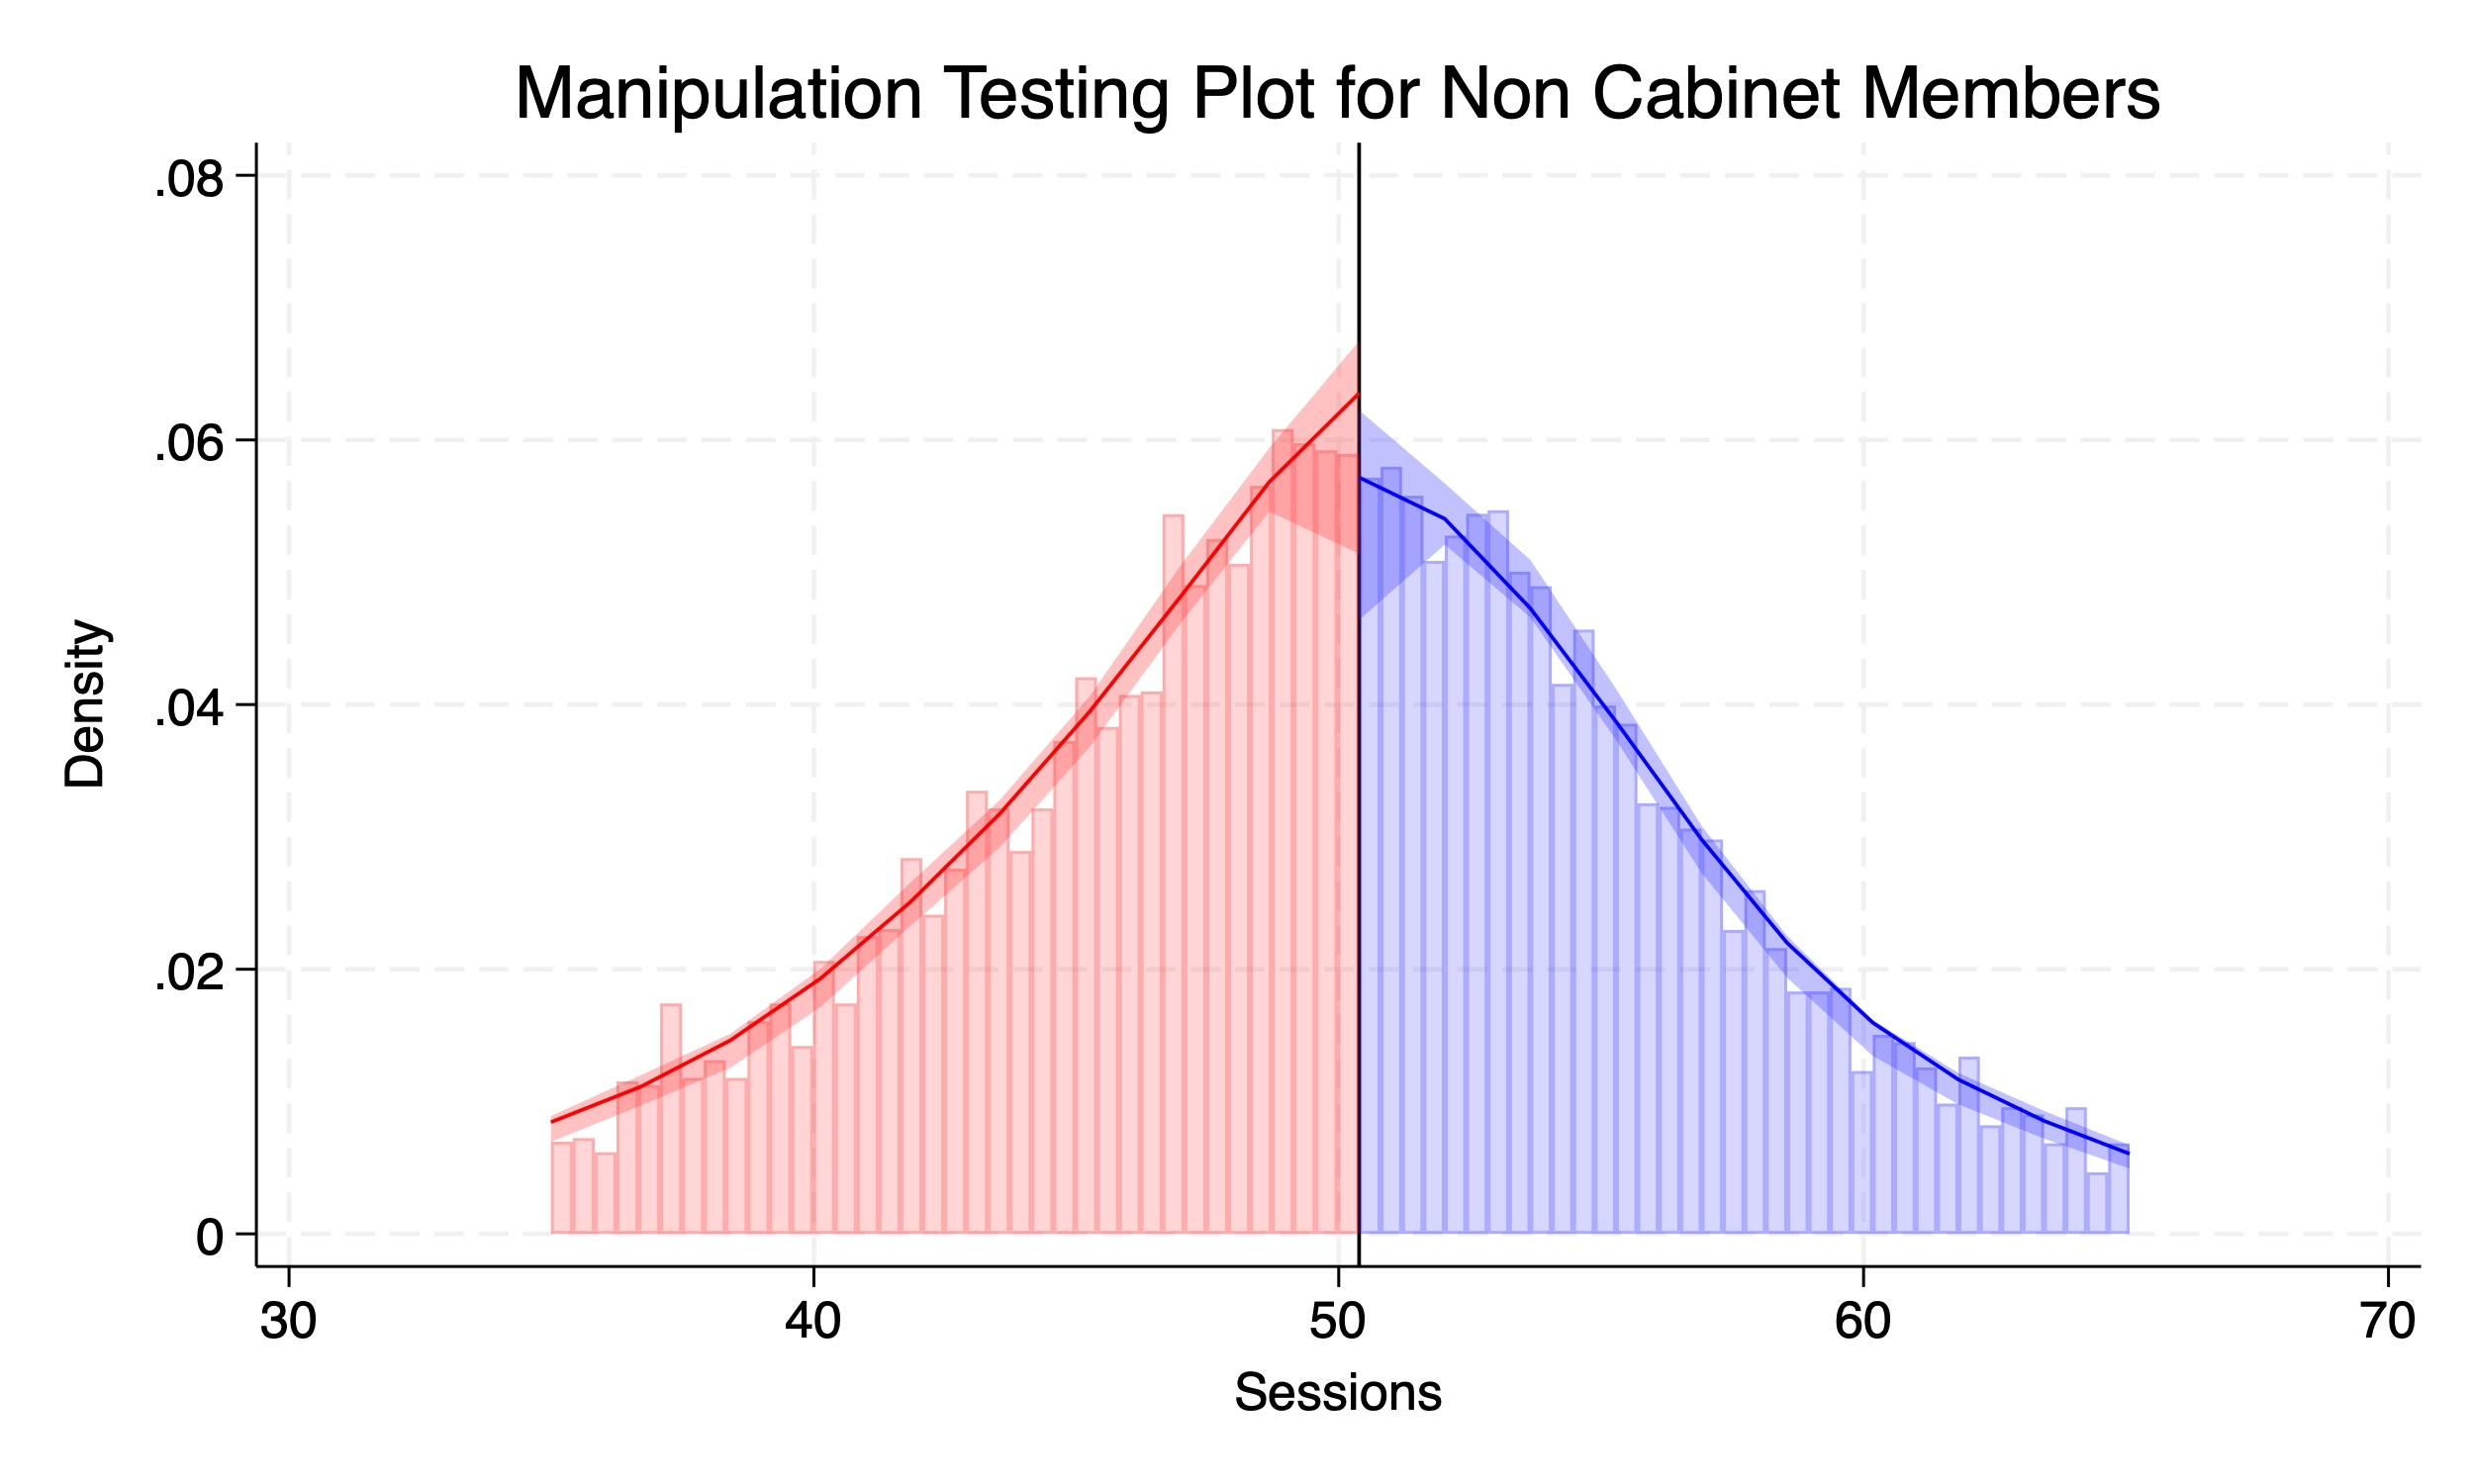
\includegraphics[width=0.8\textwidth]{images/mccrary_test_fk_read_non_cab.jpg}
    \captionof{figure}{\textit{McCrary Manipulation Test for Distribution of Non Cabinet Members around catoff off 1868 election}}
    \label{fig:mccrary_test_fk_read_non_cab}
\end{center}

\begin{center}
    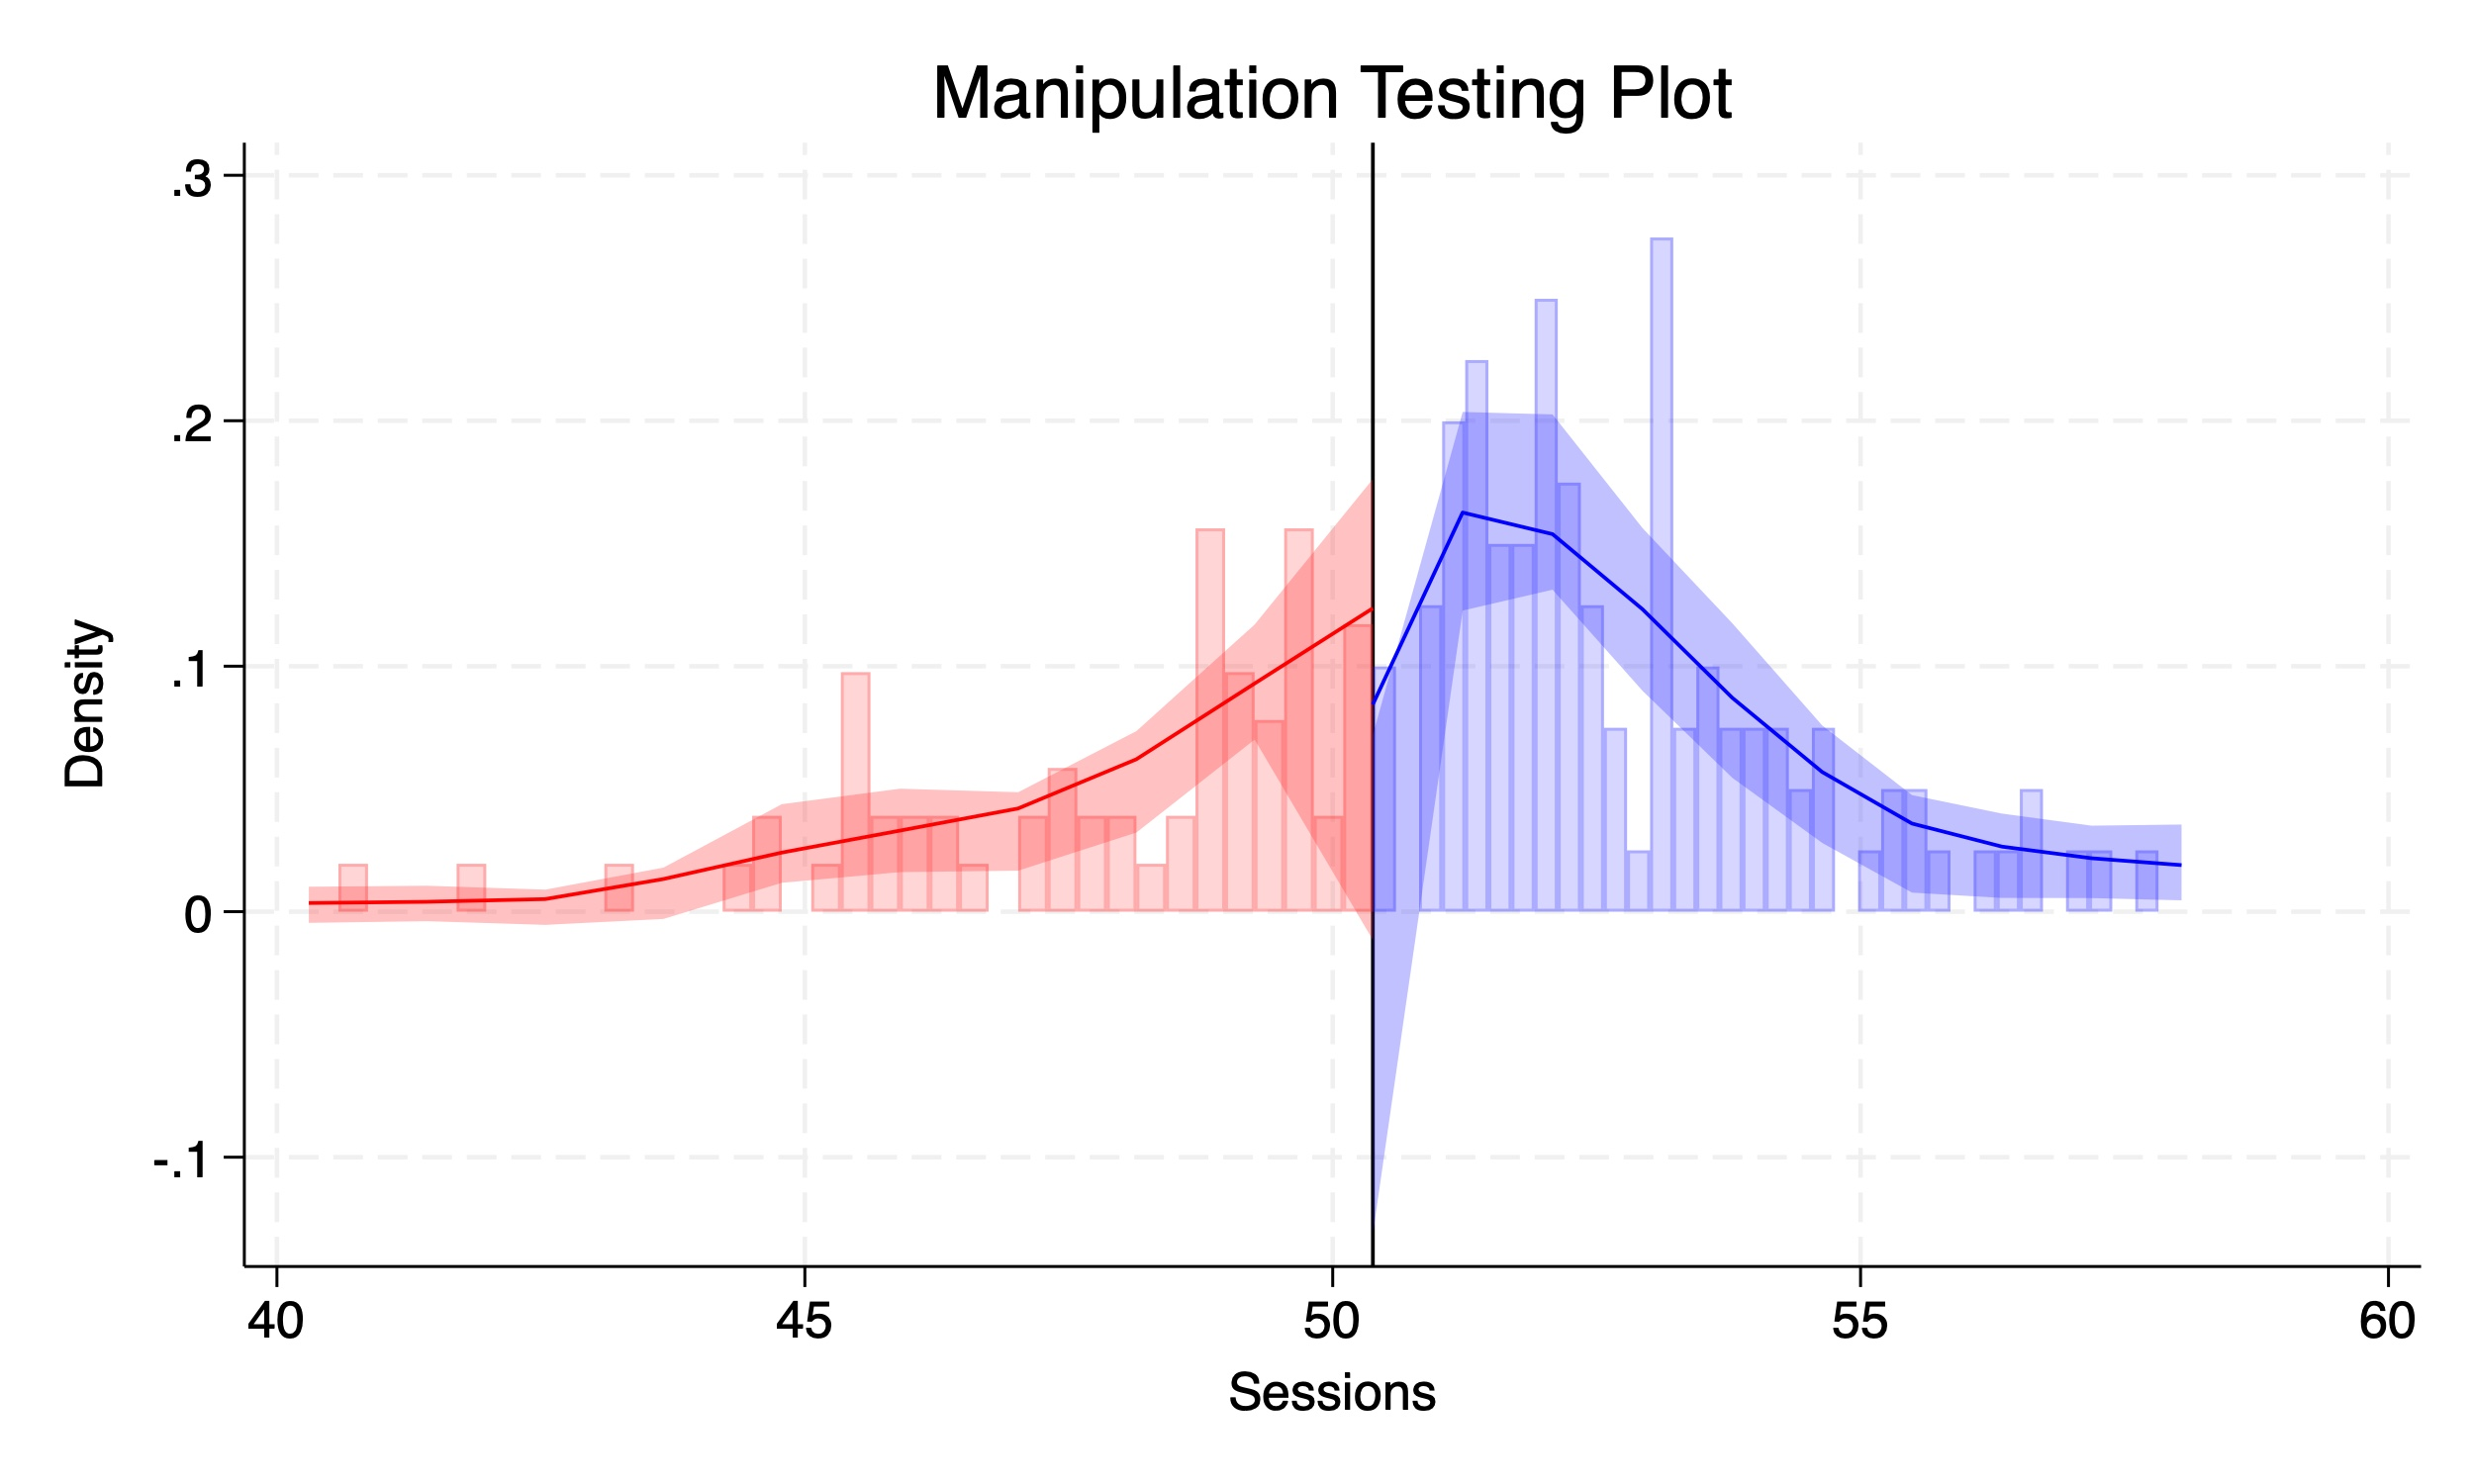
\includegraphics[width=0.7\textwidth]{images/mccrary_test_fkread.jpg}
    \captionof{figure}{\textit{McCrary Manipulation Test for Distribution of Cabinet Members around catoff off 1868 election}}
    \label{fig:mccrary_test_fkread}
\end{center}

%------- End of the File -------